\section{Discussion}\label{sec:discussion}
\paragraph{Task 4} Compare the phase velocity 

\textit{I suspect that we totally messed this up :(}

\paragraph{Task 7} \textit{Reduce the plate spacing to 4 mm and increase the width to 14 mm in the environment used for Section \ref{sec:non-ideal}.
Does the far field in the $xy$ and $yz$ planes behave like a uniform plane wave?}

Narrowing the gap between the electric field boundaries and widening them creates the propagation patterns shown in Fig. \ref{fig:narrow}.

\begin{figure}[htpb]
	\centering
	\subfigure[]
	{
		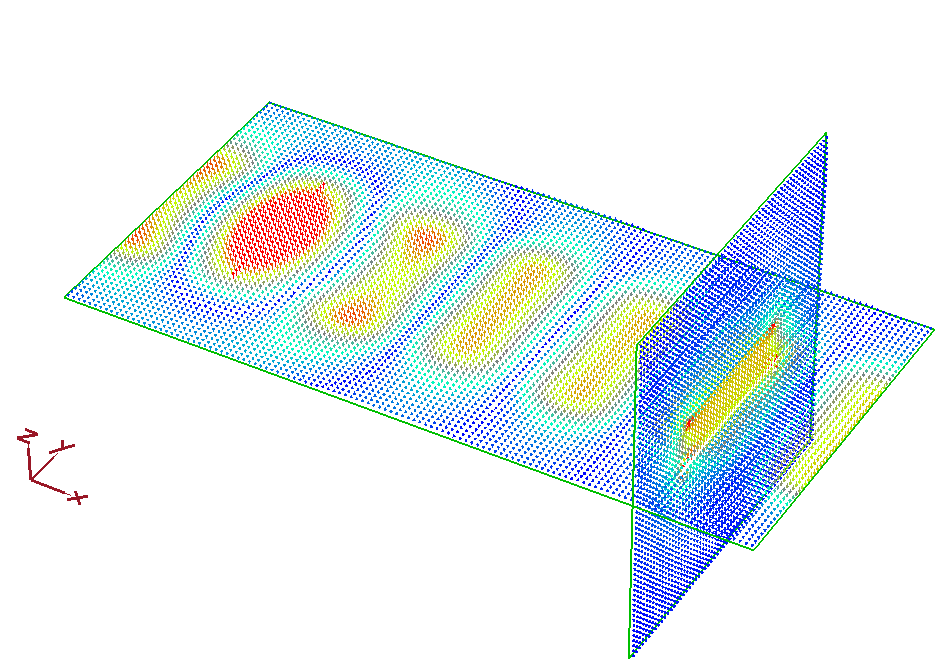
\includegraphics[width=0.575\linewidth]{graphics/Task2-3d-narrowplate}
		\label{fig:3d-narrow}
	}
	\subfigure[$yz$-orientation]
	{
		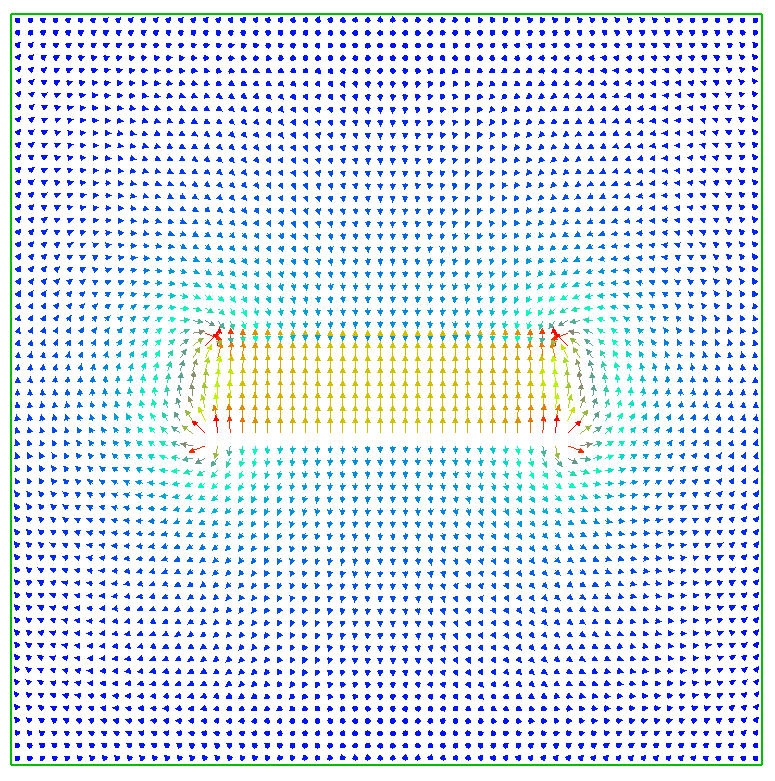
\includegraphics[width=0.375\linewidth]{graphics/Task2-yz-narrowplate}
		\label{fig:yz-narrow}
	}
	\caption{Propagation in a non-ideal, narrow parallel plate}
	\label{fig:narrow}
\end{figure}

The magnitude of the waves in Fig. \ref{fig:narrow}\subref{fig:3d-narrow} is greater than those in Fig. \ref{fig:non-ideal}\subref{fig:3d} and the groups have a much shorter and wider region of similar magnitude.
Fig. \ref{fig:narrow}\subref{fig:yz-narrow} confirms that both the direction and magnitude of the wave are similar far from the source.
Changing the electric field arrangement to make the separation smaller and boundaries wider has restored the plane wave behavior for the region between the boundaries.

\paragraph{Task 8} \textit{Determine $\alpha$ and $\beta$ for the waveguide with dielectric from Section \ref{sec:dielectric}.}

Fig. \ref{fig:Task3-mesh} can be used to determine the attenuation of the wave with equations \eqref{eqn:alpha} and \eqref{eqn:beta}.

\begin{figure}[tbph]
	\centering
	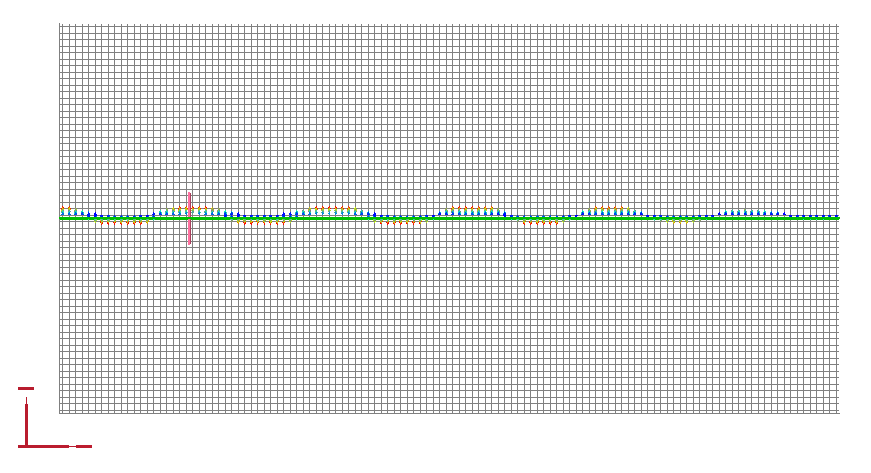
\includegraphics[width=0.7\linewidth]{graphics/Task3-mesh}
	\caption{$xz$ view of Fig. \ref{fig:Task3-3d-animation}}
	\label{fig:Task3-mesh}
\end{figure}
\begin{align}
	\alpha &= { \ln \left( { E_z(x_1) \over E_z(x_2) } \right) \over m \Delta x } \label{eqn:alpha} \\
	\beta &= { 2 \pi \over \lambda } \label{eqn:beta}
\end{align}
Choosing $x_1$ and $x_2$ as the positions of adjacent maxima, $\Delta x$ as 0.5 mm and $m$ as the number of grid squares separating $x_1$ and $x_2$ yields:

\textit{it's too small to be useful. no z scale either :(}

\paragraph{Task 9} \textit{Compare the results of Task 8 to the theoretical values.}

The attenuation and phase constants are:
\begin{align*}
	\alpha &= { \omega \sqrt{\mu \epsilon} \over \sqrt{2} } \sqrt{\sqrt{1 + \left( {\sigma \over \omega \epsilon} \right)^2} - 1} \\
	&= { \omega \sqrt{\epsilon_r} \over c_0 \sqrt{2} } \sqrt{\sqrt{1 + \left( {\sigma \over \omega \epsilon_0 \epsilon_r} \right)^2} - 1} \\
	&= { 2 \pi \cdot \SI{10}{\giga\hertz} \cdot \sqrt{4} \over c_0 \sqrt{2} } \sqrt{\sqrt{1 + \left( {0.5 \over 2 \pi \cdot \SI{10}{\giga\hertz} \cdot \epsilon_0 \cdot 4} \right)^2} - 1} \\
	&= \SI{7.39}{\neper\per\meter}
\end{align*}
\begin{align*}
	\beta &= { \omega \sqrt{\mu \epsilon} \over \sqrt{2} } \sqrt{\sqrt{1 + \left( {\sigma \over \omega \epsilon} \right)^2} + 1} \\
	&= \SI{46.80}{\radian\per\meter}
\end{align*}

\paragraph{Task 10} \textit{Modify the waves in \texttt{Polarization\_TE.mef} to produce various kinds of polarizations}

\begin{figure}[htpb]
	\centering
	\subfigure[$A = 1,\: \phi_\Delta = \SI{0}{\degree}$]
	{
		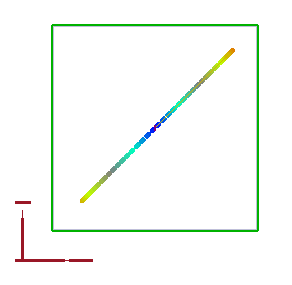
\includegraphics[width=0.475\linewidth]{graphics/Task4-lin}
		\label{fig:lin}
	}
	\subfigure[$A = 1,\: \phi_\Delta = \SI{-90}{\degree}$]
	{
		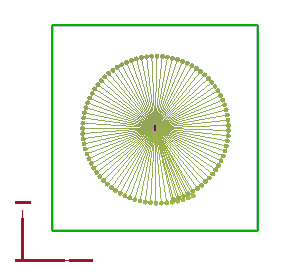
\includegraphics[width=0.475\linewidth]{graphics/Task4-RHC}
		\label{fig:RHC}
	}
	\subfigure[$A = 1,\: \phi_\Delta = \SI{45}{\degree}$]
	{
		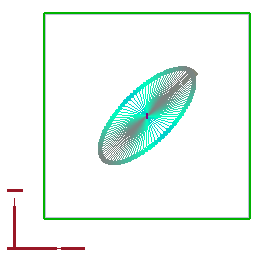
\includegraphics[width=0.475\linewidth]{graphics/Task4-LHE}
		\label{fig:LHE}
	}
	\caption{Various polarizations of a propagating electric field}
	\label{fig:polarization}
\end{figure}

Fig. \ref{fig:polarization} shows the result of changing $E_x$ and $E_y$. 
